% figures/many-to-many.tex
\documentclass[11pt]{article}
\usepackage[margin=1.5cm]{geometry}
\usepackage{tikz}
\usetikzlibrary{positioning,shapes.geometric,arrows.meta,calc}
\pagestyle{empty}
\begin{document}
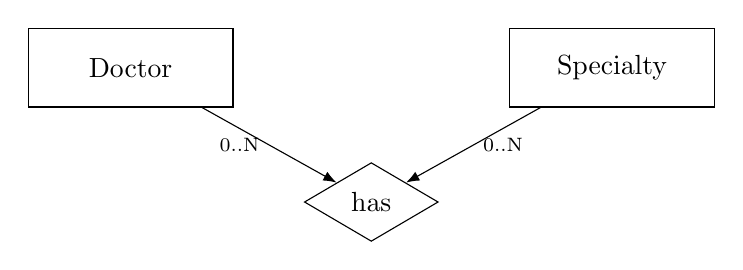
\begin{tikzpicture}[node distance=18mm, >=Latex]
  \node[draw, rectangle, minimum width=2.6cm, minimum height=1cm] (A) {Doctor};
  \node[draw, rectangle, minimum width=2.6cm, minimum height=1cm, right=35mm of A] (B) {Specialty};
  \node[draw, diamond, aspect=2, minimum width=1.6cm, minimum height=1cm, below=12mm of $(A)!0.5!(B)$] (R) {has};

  \draw[->] (A) -- (R) node[midway, left, font=\scriptsize] {0..N};
  \draw[->] (B) -- (R) node[midway, right, font=\scriptsize] {0..N};
\end{tikzpicture}
\end{document}
